
\documentclass[paper=a4, fontsize=11pt]{scrartcl} % A4 paper and 11pt font size

\usepackage{times, epsfig, graphicx, amsmath, amssymb, floatrow, booktabs, url, multirow,comment}
\usepackage{graphicx}
\graphicspath{ {images/} }
\usepackage[T1]{fontenc} % Use 8-bit encoding that has 256 glyphs
\usepackage{fourier} % Use the Adobe Utopia font for the document - comment this line to return to the LaTeX default
\usepackage[english]{babel} % English language/hyphenation
\usepackage{amsmath,amsfonts,amsthm} % Math packages
\usepackage{hyperref}
\usepackage{sectsty} % Allows customizing section commands
%\allsectionsfont{\centering \normalfont\scshape} % Make all sections centered, the default font and small caps

\usepackage{fancyhdr} % Custom headers and footers
\pagestyle{fancyplain} % Makes all pages in the document conform to the custom headers and footers
\fancyhead{} % No page header - if you want one, create it in the same way as the footers below
\fancyfoot[L]{} % Empty left footer
\fancyfoot[C]{} % Empty center footer
\fancyfoot[R]{\thepage} % Page numbering for right footer
\renewcommand{\headrulewidth}{0pt} % Remove header underlines
\renewcommand{\footrulewidth}{0pt} % Remove footer underlines
\setlength{\headheight}{1.6pt} % Customize the height of the header


\numberwithin{equation}{section} % Number equations within sections (i.e. 1.1, 1.2, 2.1, 2.2 instead of 1, 2, 3, 4)
\numberwithin{figure}{section} % Number figures within sections (i.e. 1.1, 1.2, 2.1, 2.2 instead of 1, 2, 3, 4)
\numberwithin{table}{section} % Number tables within sections (i.e. 1.1, 1.2, 2.1, 2.2 instead of 1, 2, 3, 4)

\setlength{\parindent}{2ex} % Removes all indentation from paragraphs - comment this line for an assignment with lots of text

%----------------------------------------------------------------------------------------
%   TITLE SECTION
%----------------------------------------------------------------------------------------

\newcommand{\horrule}[1]{\rule{\linewidth}{#1}} % Create horizontal rule command with 1 argument of height

\title{ 
\normalfont \normalsize 
\textsc{Indraprastha Institute of Information Technology, Delhi} \\ [1pt] % Your university, school and/or department name(s)
\horrule{0.1pt} \\[0.2cm] % Thin top horizontal rule
\huge Extreme Learning Machine for Collaborative Filtering \\ % The assignment title
\horrule{0.2pt} \\[0.2cm] % Thick bottom horizontal rule
}

\author{Sagar Verma \\ MT15056} % Your name

\date{\normalsize\today} % Today's date or a custom date

\begin{document}

\maketitle % Print the title

%----------------------------------------------------------------------------------------
%   PROBLEM 1
%----------------------------------------------------------------------------------------

\section{Cold Start Problem}


\par
Cold start problem in collaborative filtering is predicting information of a new user when that user has not rated any item. Cold start problem is usually solved by using metadata information of user and item.

\section{Extreme Learning Machine}

\begin{figure}[H]
\centering
    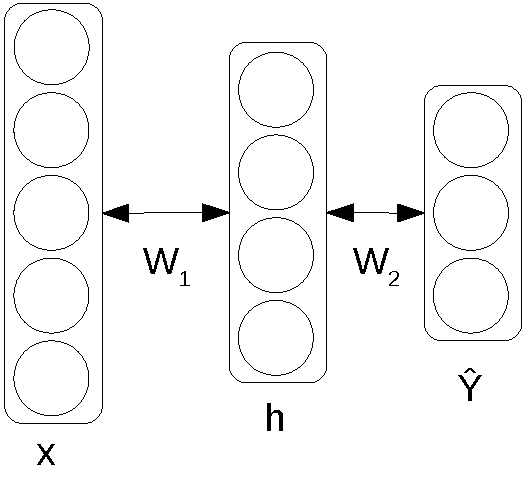
\includegraphics[width=0.35\linewidth]{ELM}
    \caption{A basic ELM with one hidden layer.}
\end{figure}

\par
Extreme learning machine(ELM) are a type of feedforward neural network used to solve classification or regression problems. The ELM network contains a single layer of hidden nodes. Weights connecting inputs to hidden nodes are randomly assigned and never updated. These weights between hidden nodes and outputs are learned in a single step. ELMs have been shown to perform good on certain class of problems were a linear model has to be learned and they achieve accuracy similar to models learned with backpropagation and at thousands times faster speed. The simplest ELM training algorithm takes the form

\begin{equation}
   \hat{Y} = W_2 \sigma (W_1x)
\end{equation}

where $w_1$ is the matrix of input-to-hidden layer weights, $\sigma$ is activation function and $W_2$ is the matrix of hidden-to-output-layer weights.

Types of activation function

\begin{enumerate}
    \item \textit{\textbf{Linear}} : $f(x) = x$
    \item \textit{\textbf{Sigmoid}} : $f(x) = \frac{1}{1+e^{-x}}$
    \item \textit{\textbf{Tanh}} : $f(x) = tanh(x) = \frac{2}{1+e^{-2x}} - 1$
    \item \textit{\textbf{Radial basis function}} : $f(x) = \sum_{i=1}^{N} a_i \rho(||x-c_i||)$ 
            where $N$ is the number of neurons in the hidden layer, $c_i$ is the center vector of neuron $i$ and $a_i$ is the weight of neuron $i$ in the linear output neuron. $\rho(||x-c_i||)$ is norm function given by,

            \begin{enumerate}
                \item \textit{\textbf{rbf\_l1}} : $\rho(||x-c_i||) = exp[-\beta \; ||x-c_i||]$
                \item \textit{\textbf{rbf\_l2}} : $\rho(||x-c_i||) = exp[{-\beta \; ||x-c_i||}^{2}]$
                \item \textit{\textbf{rbf\_linf}} : $\rho(||x-c_i||) = exp[{-\beta \; min(||x-c_i||})]$
            \end{enumerate}
\end{enumerate}


\section{ELM to solve cold start problem in collaborative filtering}

\par
To use ELM to solve cold start problem we need to treat it as classification problem. In this cas user metadata and item metadata form features for the ELM and label is the rating itself. For any new user we find all item ratings by giving user and item metadata as input to trained model. Each column of metadata is encoded as one-hot vector and similarly label is encoded as one-hot vector. For user cold start problem we have some item ratings from some of the users, ELM is trained on those values and prediction is done for completely new users. For item cold start problem we have some item ratings from some of the users, ELM is trained on those values and prediction is done for completely new items.

Different activation functions are tried to find best perceptron activation function. Different number of hidden nodes between 5 and 50 are used with stride of 5. Average result for all values is reported in the table \ref{table:results}.

\begin{table}
\centering
\begin{tabular}{l c c c c c c} \toprule[0.2mm]
\multirow{2}{*}{\textbf{Function}} & \multicolumn{3}{c}{\textbf{User cold start}} & \multicolumn{3}{c}{\textbf{Item cold start}} \\ \cmidrule{2-7}
& \textbf{RMSE} & \textbf{NMAE} & \textbf{\#Nodes} & \textbf{RMSE} & \textbf{NMAE} & \textbf{\#Nodes} \\ \midrule
\textbf{linear} & 1.2190 & 0.2234 & 10 & 1.2024 & 0.2216 & 45 \\
\textbf{sigmoid} & 1.2054 & 0.2221 & 30 & 1.2032 & 0.2218 & 45 \\
\textbf{tanh} & 1.2048 & 0.2223 & 50 & 1.2068 & 0.2223 & 50 \\
\textbf{rbf\_l1} & 1.2145 & 0.2227 & 20 & 1.2176 & 0.2233 & 45 \\
\textbf{rbf\_l2} & 1.2016 & 0.2223 & 50 & 1.2028 & 0.2218 &  50 \\
\textbf{rbf\_linf} & 1.2189 & 0.2223 & 35 & 1.1977 & 0.2208 & 45 \\
\bottomrule[0.2mm]
\end{tabular}
\caption{Results for user and item cold start problem. Different types of perceptron activation function have been used. Results are reported for best number of nodes in the hidden layer.}
\label{table:results}
\end{table}

\renewcommand{\tabcolsep}{0.01cm}
\begin{figure}
\begin{tabular}{cc}
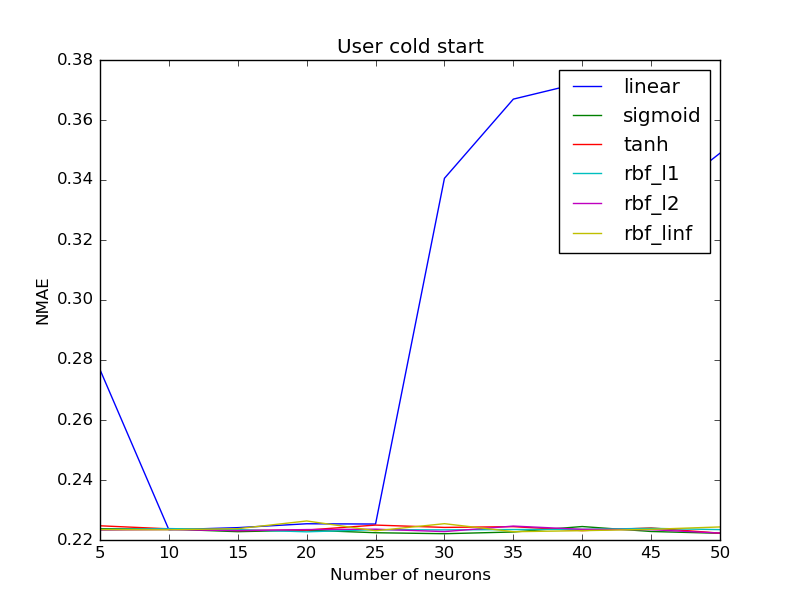
\includegraphics[width=0.5\linewidth]{users} &
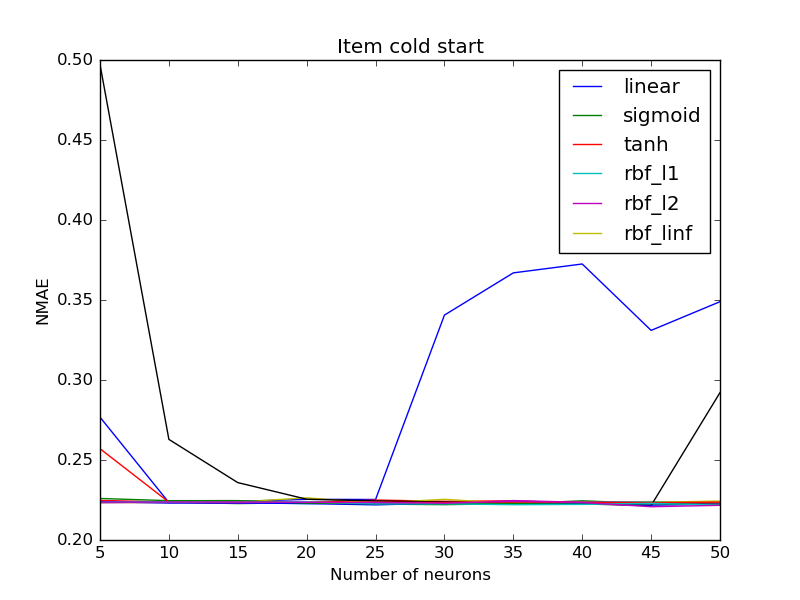
\includegraphics[width=0.5\linewidth]{items} \\
\end{tabular}
\caption{Left figure shows how different perceptron activation function perform with number of hidden nodes. Between 10-25 number of nodes every type of activation function is able to learn and give best performance for `user cold start' problem. For `item cold start' problem number of nodes between 20-25 gives best performance for all types of activation functions. Its evident that linear activation function performs very poorly and `radial basis functions' perform best in both cases.}
\label{fig:neuron_vs_nmae}
\end{figure}

\end{document}